\chapter{TileCal Data Quality}\label{app:Tile-DQ}
	This appendix gives an overview of the \gls{TileCal} and \gls{ATLAS} \gls{DQM} systems. The author served as \gls{DQ} Co-Coordinator for a significant portion of their time in the Ph.D. program. During their tenure, it was their responsibility to verify the integrity and sign off on all physics data coming out of \gls{TileCal}. 

	\section{ATLAS Data Quality}
		The process of data collection with the \gls{ATLAS} detector begins with an \gls{LHC} fill. Each fill corresponds to injections of protons into the \gls{LHC} in preparation for data taking. When the beams are collimated and focused, the \gls{LHC} team declares a period of ``stable beams''. At this point, the \gls{ATLAS} team begins to ramp up the high voltage in the tracker and muon systems. Once the pixel preamplifiers are turned on, \gls{ATLAS} declares ``ready for physics''. Data collected by \gls{ATLAS} is recorded against a six digit number referred to as a run number. Each run is subdivided into \glspl{LB}, with each \gls{LB} corresponding to 60 seconds of data taking. \glspl{LB} provide a granularity for checking quality of data and sorting of data based on its quality. 


	\section{Calibration Systems}
		To ensure the data being collected by \gls{TileCal} is accurate and meets the required standards a series of calibration checks are performed with varying frequency. The systems used for calibration were designed to be built into the full detector; allowing calibration between physics data taking runs without requiring physical access to the detector. A diagram of the various calibration systems and where in the readout chain each calibration is done can be seen in Figure \ref{fig:tile-calib-chain}.

		\begin{figure}
			\centering
			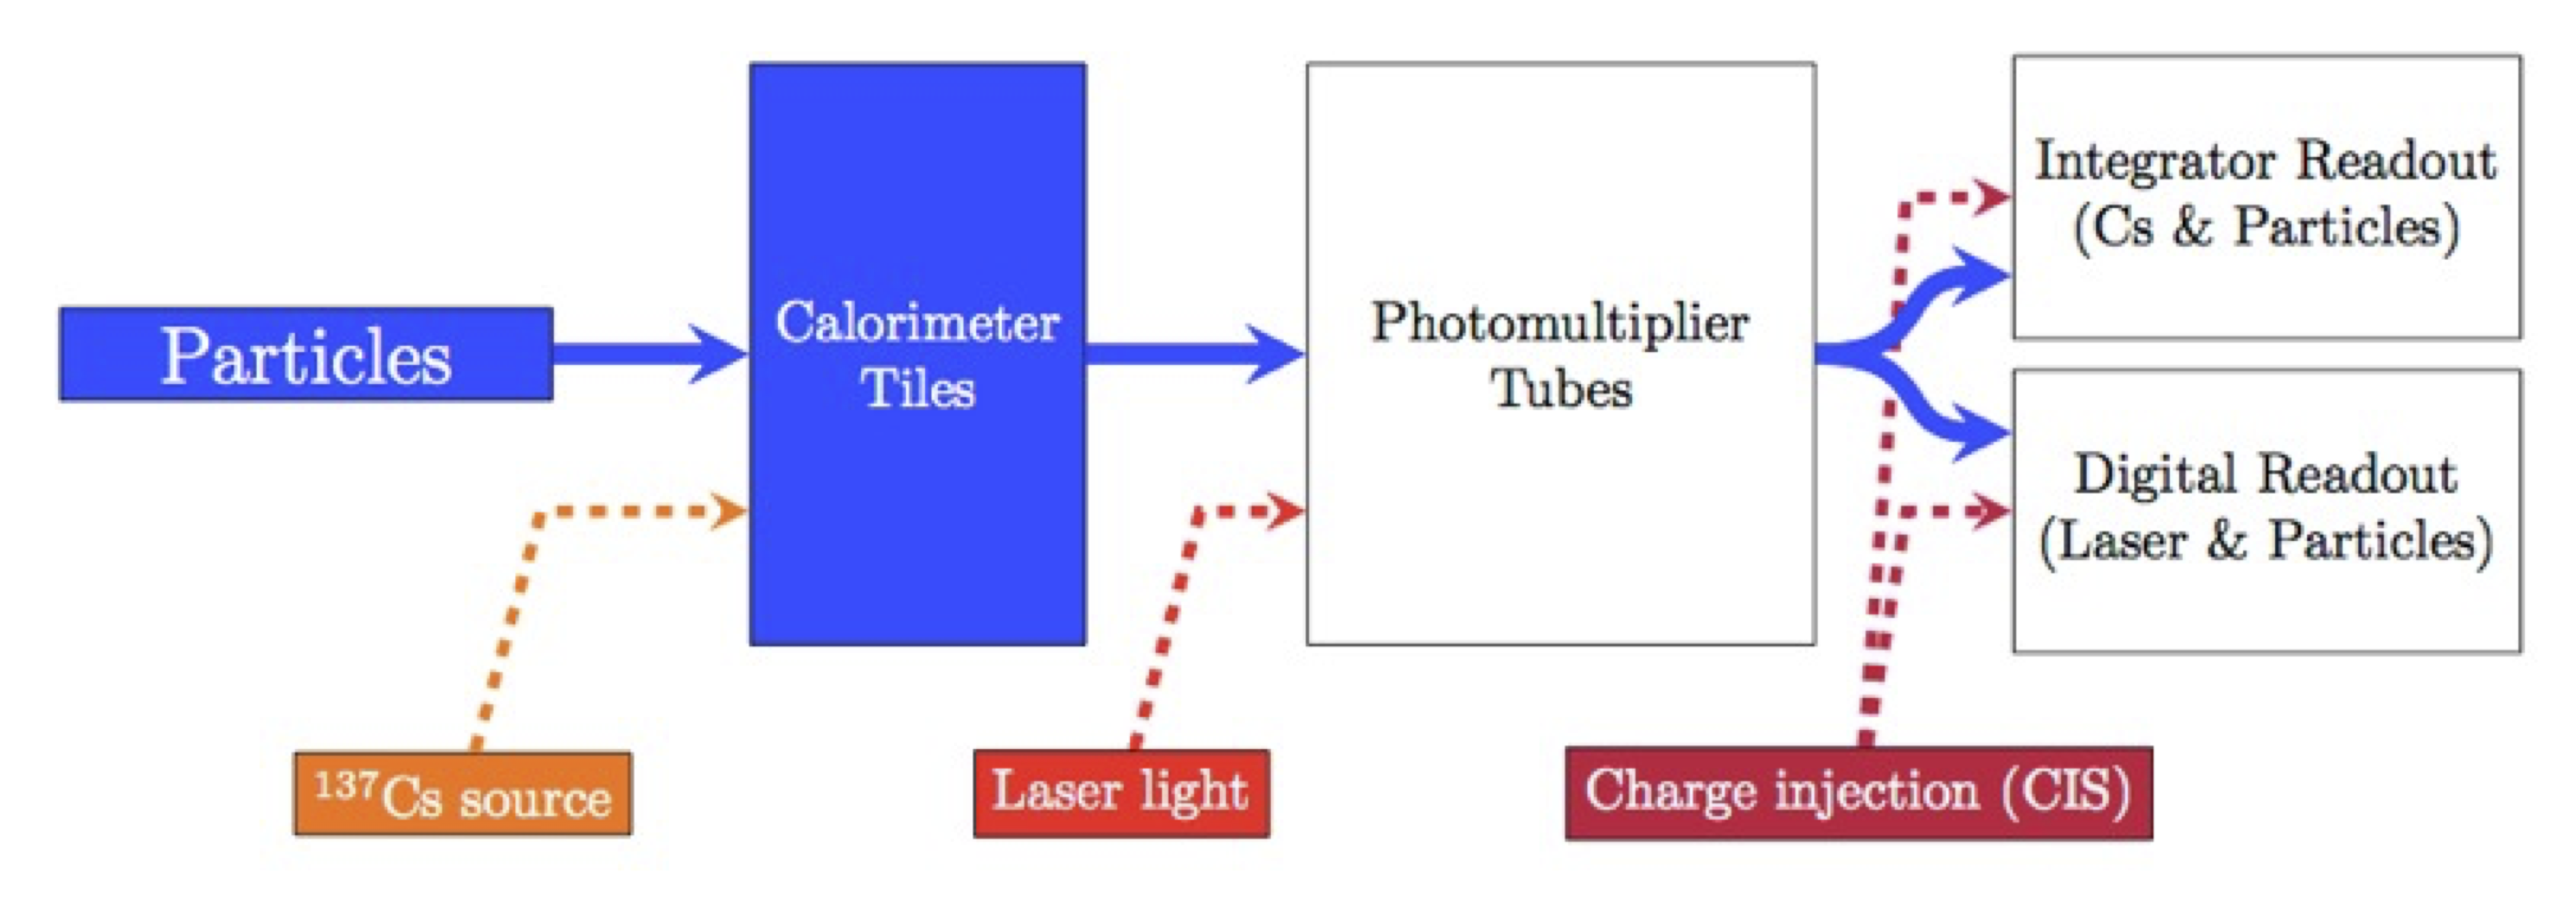
\includegraphics[width=.75\textwidth,keepaspectratio=true]{appendices/images/Tile_Calibration_Diagram.png}
			\caption{\label{fig:tile-calib-chain} \gls{TileCal} calibration checks within the readout chain \cite{ATLAS-tile}.}
		\end{figure}

		The cesium calibration system within \gls{TileCal} is meant to calibrate the entire readout chain from scintillator to final digital signal readout. Several sources of $\mathrm{CS}^{137}$ are hydraulically moved throughout the detector. The cesium calibration was designed to be run once a month\footnote{Due to historical issues with leaking hydraulic fluid, the frequency of cesium scans was drastically reduced during Run-2.}. The laser calibration system measures the response of the \glspl{PMT} with respect to the last cesium scan. Laser calibration can be done during empty bunches within the \gls{LHC} fill and with dedicated calibration runs as well. The \gls{CIS} measures the response of digitizers and readout electronics by injecting controlled charges into the electronics. \gls{CIS} calibration is done with dedicated calibration runs. The last calibration system is the minimum bias system, where physics signal is integrated over $\sim 10 - 20 $ ms. Minimum bias calibration is used to fill in the gaps between cesium calibration scans. The average response variation for one cell from the laser, cesium, and minimum bias systems can be seen in Figure \ref{fig:tile-calib-a13}. 

		\begin{figure}
			\centering
			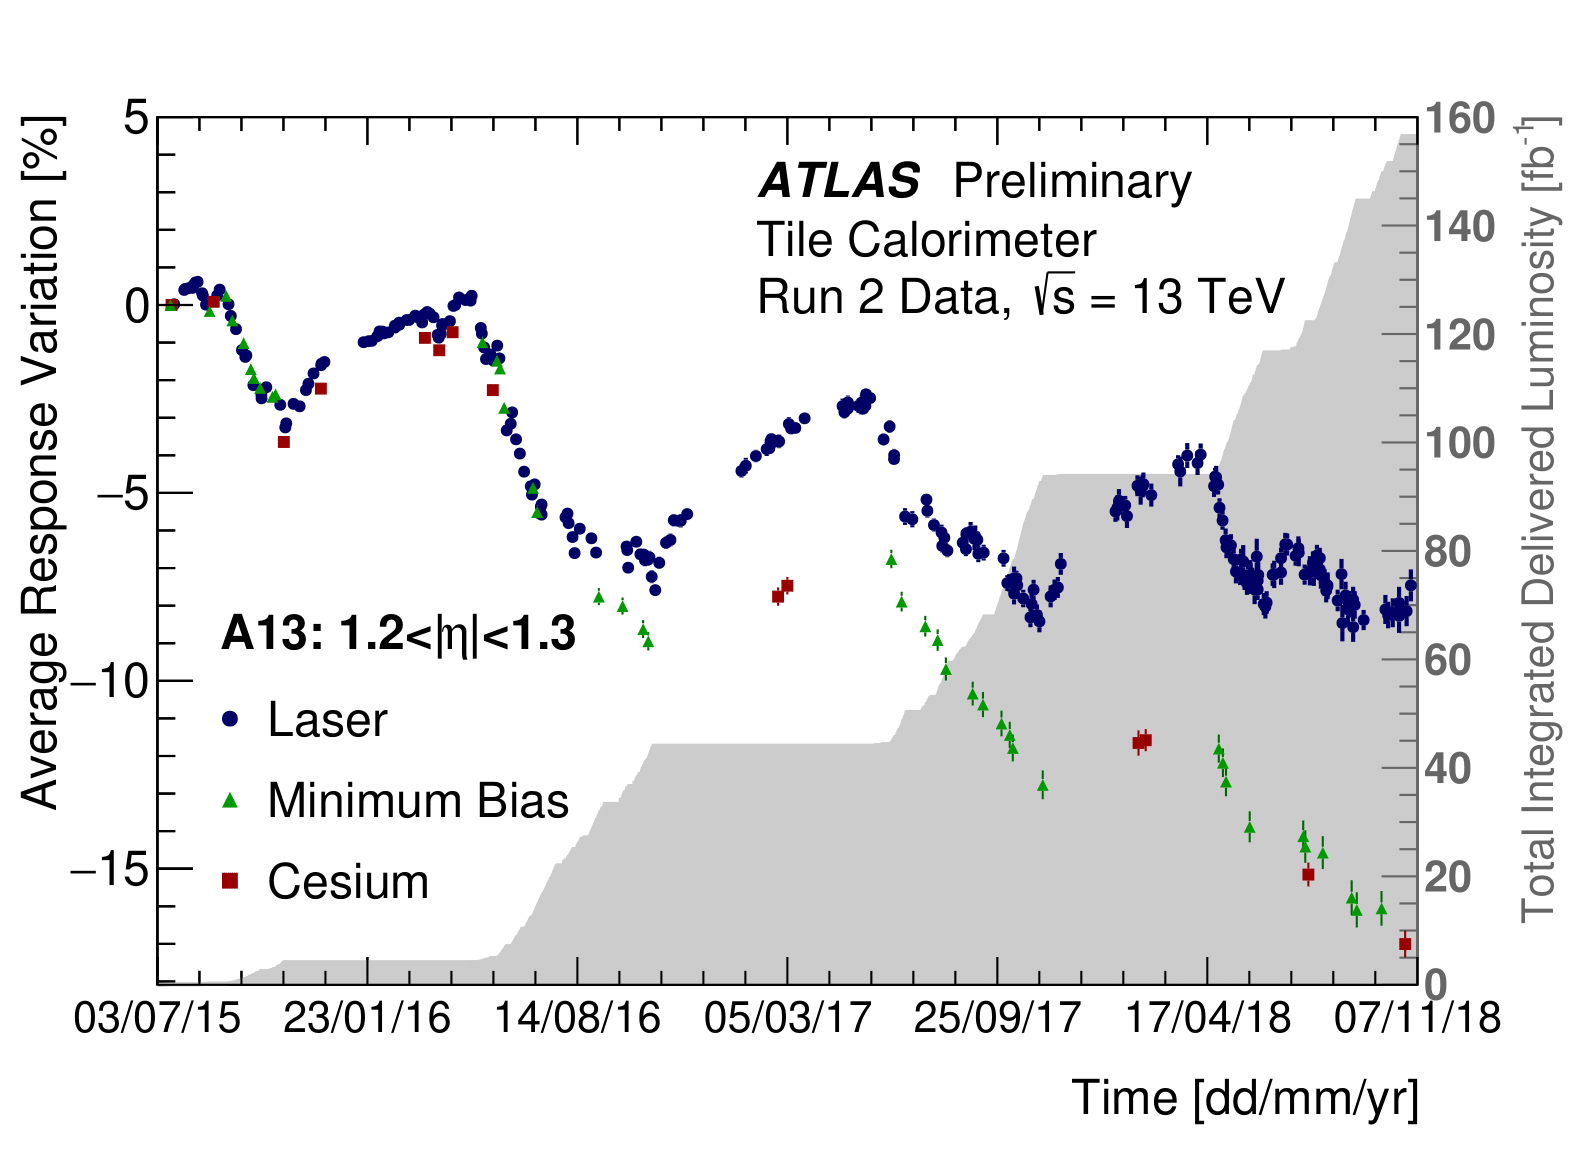
\includegraphics[width=.75\textwidth,keepaspectratio=true]{appendices/images/A13_run2.png}
			\caption{\label{fig:tile-calib-a13} Average response variation from the beginning of Run-2 of \gls{TileCal} cell A13 is shown \cite{Tile-Run2-perf}. }
		\end{figure}

		Calibration constants are extracted from each calibration system and stored in a central ATLAS conditions database. Bookkeeping is done with an \gls{IOV} that corresponds to specific \glspl{LB} within a run. The energy reconstructed at the \gls{EM} scale is 
		\begin{equation}
		E = \frac{A [ADC \, Counts]}{ C_{Cs} \cdot C_{Las} \cdot C_{CIS} [ADC \, counts/pC] \cdot C_{TB} [pC/GeV] }
		\end{equation}
		where A is the amplitude of the PMT signal after it has been shaped, amplified, and digitized at 40 MHz with 10-bit \glspl{ADC} and $C_{TB}$ is a calibration constant that was determined at dedicated test beams.


	\section{TileCal Data Quality}
		Quality of data is monitored both online and offline; a schematic of the path of data can be seen in Figure \ref{fig:dq-data-flow}. Online monitoring offers real time feedback on the data being collected, whereas offline monitoring is delayed but more detailed. Approximately 10\% of collision events are quickly reconstructed in an express data stream. The data in this express stream is reviewed within 48 hours to allow subsystems an opportunity to change calibration constants and/or mask channels deemed bad. Figure \ref{fig:tile-masked-cells} shows the evolution of \gls{TileCal} masked channels and cells throughout Run-2. After the 48 hour window, the full run is reconstructed using the updated conditions and once again reviewed by subsystem experts. The subsystem experts then approve the data or reject it based on a combination of automated test and human judgement. Figure \ref{fig:dq-run2-lumi} shows the amount of collected luminosity throughout Run-2 and how much of it passes the ``good for physics'' requirements and Figure \ref{fig:dq-run2-efficiency} shows the overall efficiency of the whole ATLAS detector. Figure \ref{fig:dq-run2-inefficiencies} shows the inefficiencies by subsystem. For the whole of Run-2 \gls{TileCal} was 99.65\% efficient in terms of data quality.

		\begin{figure}
			\centering
			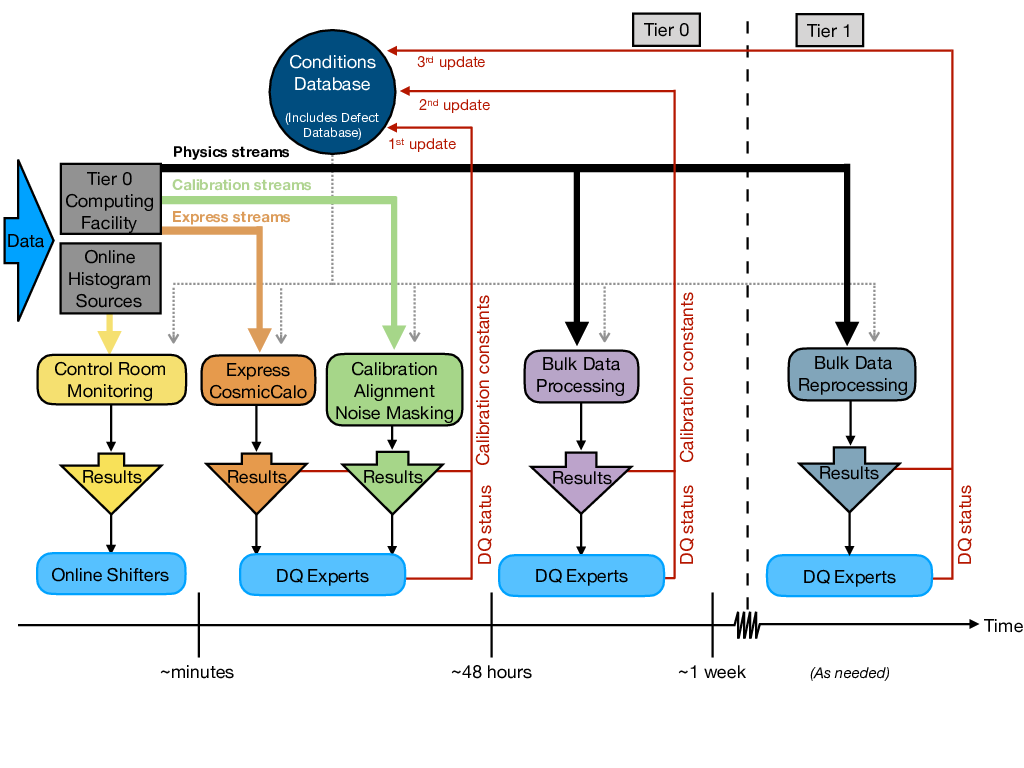
\includegraphics[width=.75\textwidth,keepaspectratio=true]{appendices/images/DQ_Data_Flow_Diagram.png}
			\caption{\label{fig:dq-data-flow} Schematic diagram illustrating the nominal Run-2 operations workflow for the data quality assessment of ATLAS data. Online histogram sources include the high-level trigger farm, the data acquisition system, and full reconstruction of a fraction of events accepted by the trigger \cite{DQ-Run2}.}
		\end{figure}

		\begin{figure}
			\centering
			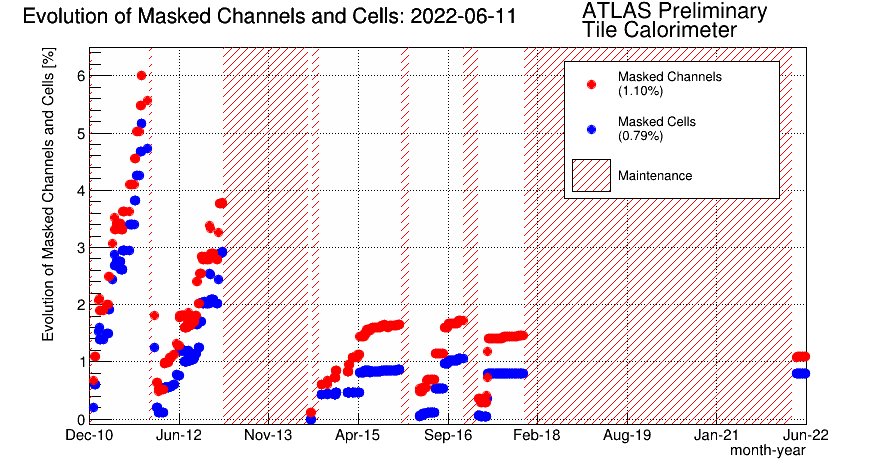
\includegraphics[width=.75\textwidth,keepaspectratio=true]{appendices/images/Masked_Cells_timeline_2022.png}
			\caption{\label{fig:tile-masked-cells} Evolution of masked \gls{TileCal} cells during Run-2 \cite{Tile-Run2-perf}.}
		\end{figure}

		\begin{figure}
			\centering
			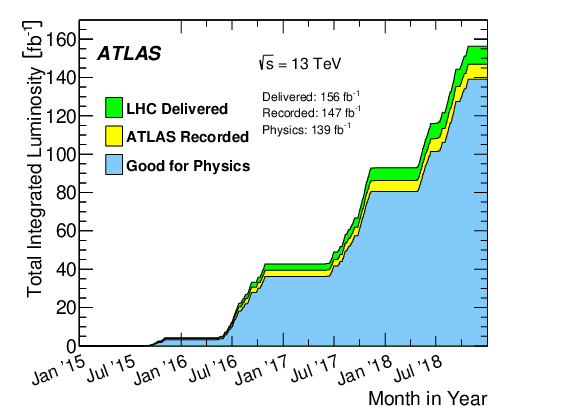
\includegraphics[width=.75\textwidth,keepaspectratio=true]{appendices/images/ATLAS_DQ_lumi.png}
			\caption{\label{fig:dq-run2-lumi} Cumulative integrated luminosity delivered to and recorded by ATLAS between 2015 and 2018 during stable beam pp collision data-taking at \sqs. This includes machine commissioning periods, special runs for detector calibration, and LHC fills with a low number of circulating bunches or bunch spacing greater than 25 ns. Also shown is the cumulative integrated luminosity certified for physics analysis usage for the ATLAS experiment between 2015 and 2018 during standard pp collision data-taking at \sqs. The total integrated luminosity recorded for the standard \sqs \pp collision dataset corresponds to 145 \ifb. It is this number that is used in the denominator when calculating the data quality efficiency of the standard \sqs \pp collision dataset \cite{DQ-Run2}.}
		\end{figure}

		\begin{figure}
			\centering
			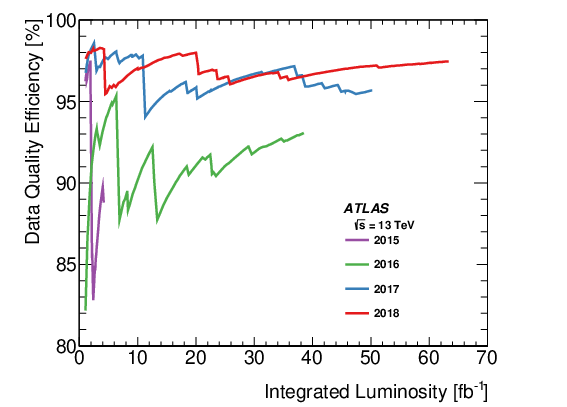
\includegraphics[width=.75\textwidth,keepaspectratio=true]{appendices/images/ATLAS_DQ_Run2_DQ_Efficiency.png}
			\caption{\label{fig:dq-run2-efficiency} Cumulative data quality efficiency versus total integrated luminosity delivered to the ATLAS experiment between 2015 and 2018 \cite{DQ-Run2}.}
		\end{figure}

		\begin{figure}
			\centering
			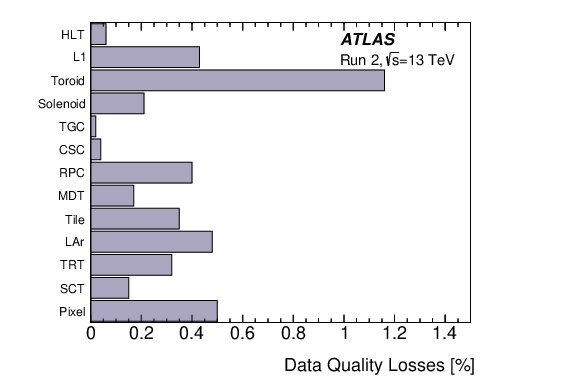
\includegraphics[width=.75\textwidth,keepaspectratio=true]{appendices/images/DQ_Inefficiencies.png}
			\caption{\label{fig:dq-run2-inefficiencies} Luminosity-weighted data quality inefficiencies (in \%) during stable beams in standard pp collision physics runs at \sqs between 2015 and 2018. Taken from Reference \cite{DQ-Run2}.}
		\end{figure}


